\documentclass[aspectratio=169, 11pt]{beamer}

% =========================================================================
% -- PACKAGES -------------------------------------------------------------
% =========================================================================
\usepackage{amsmath, amssymb}
\usepackage{booktabs}
\usepackage{graphicx}
\usepackage{xcolor}
\usepackage{tikz}
\usetikzlibrary{arrows.meta, positioning, shapes.geometric}
\usepackage{pgfplots}
\pgfplotsset{compat=1.17}
\usepackage{ragged2e}
\usepackage{setspace}
\usepackage[square,numbers,sort&compress]{natbib}
\usepackage{url}
\usepackage{caption}
\usepackage{etoolbox}

% =========================================================================
% -- COLOR DEFINITIONS ----------------------------------------------------
% =========================================================================
\definecolor{accent}{HTML}{005296}
\definecolor{accentlight}{HTML}{E8F0FE}
\definecolor{darktext}{HTML}{1A1A2E}
\definecolor{graytext}{HTML}{4A4A5A}
\definecolor{lightgray}{HTML}{F5F5F7}

% =========================================================================
% -- THEME & VISUAL STYLE -------------------------------------------------
% =========================================================================
\usetheme{default}
\usecolortheme{dove}
\usefonttheme{professionalfonts}

% Background & text colors
\setbeamercolor{background canvas}{bg=white}
\setbeamercolor{normal text}{fg=darktext}
\setbeamercolor{frametitle}{fg=accent, bg=white}
\setbeamercolor{title}{fg=darktext}
\setbeamercolor{subtitle}{fg=accent}
\setbeamercolor{author}{fg=graytext}
\setbeamercolor{institute}{fg=graytext}
\setbeamercolor{date}{fg=graytext}
\setbeamercolor{structure}{fg=accent}

% List styling
\setbeamercolor{itemize item}{fg=accent}
\setbeamercolor{itemize subitem}{fg=darktext}
\setbeamercolor{itemize subsubitem}{fg=graytext}
\setbeamercolor{enumerate item}{fg=accent}
\setbeamercolor{enumerate subitem}{fg=darktext}

% Block styling
\setbeamercolor{block title}{fg=white, bg=accent}
\setbeamercolor{block body}{fg=darktext, bg=accentlight}
\setbeamercolor{block title alerted}{fg=white, bg=accent}
\setbeamercolor{block body alerted}{fg=darktext, bg=accentlight}

% Alert & emphasis
\setbeamercolor{alerted text}{fg=accent}

% =========================================================================
% -- FONT SETTINGS ---------------------------------------------------------
% =========================================================================
\setbeamerfont{normal text}{size=\small}
\setbeamerfont{frametitle}{size=\Large, series=\bfseries}
\setbeamerfont{framesubtitle}{size=\normalsize, series=\mdseries}
\setbeamerfont{title}{size=\LARGE, series=\bfseries}
\setbeamerfont{subtitle}{size=\large, series=\mdseries}
\setbeamerfont{author}{size=\normalsize}
\setbeamertemplate{itemize item}{\color{accent}\textbullet}
\setbeamertemplate{itemize subitem}{\color{darktext}--}
\setbeamertemplate{itemize subsubitem}{\color{graytext}$\circ$}

% =========================================================================
% -- SPACING & LAYOUT -----------------------------------------------------
% =========================================================================
\setlength{\itemsep}{0.35em}
\setlength{\parskip}{0.2em}
\setlength{\leftmargini}{1.5em}
\setlength{\leftmarginii}{1.5em}
\setlength{\leftmarginiii}{1.5em}

% Remove navigation symbols
\setbeamertemplate{navigation symbols}{}

% Professional footer: page number only
\setbeamertemplate{footline}{%
  \hfill\textcolor{graytext}{\insertframenumber/\inserttotalframenumber}\hspace{1.2em}\vspace{0.6em}%
}

% Block styling
\setbeamertemplate{blocks}[rounded][shadow=false]

% Justified text
\justifying

% Force exact PDF page size to 1920x1080 pixels
\pdfpagewidth=1920bp
\pdfpageheight=1080bp

% =========================================================================
% -- CAPTION SETUP (Bottom-aligned, professional) -------------------------
% =========================================================================
\captionsetup[figure]{labelformat=empty,font=scriptsize,skip=2pt,justification=centering}
\captionsetup[table]{labelformat=empty,font=scriptsize,skip=2pt,justification=centering}

% =========================================================================
% -- CUSTOM ENVIRONMENTS --------------------------------------------------
% =========================================================================
% Slide with figure: content centered, caption always at bottom
\newenvironment{figslide}[1]{%
  \begin{frame}{#1}%
  \vspace{-0.3em}%
}{%
  \end{frame}%
}

% Slide with table: content centered, caption always at bottom
\newenvironment{tableslide}[1]{%
  \begin{frame}{#1}%
  \vspace{-0.3em}%
}{%
  \end{frame}%
}

% =========================================================================
% -- METADATA -------------------------------------------------------------
% =========================================================================
\title{Real-Time Adaptive Passenger Flow Prediction:\\A Hybrid Model Approach}
\subtitle{Master's Thesis Defense}
\author{Diar Begisbayev\\[0.3em]{\small Supervisor: Aivar Sakhipov}}
\institute{School of Computer Science and Engineering\\Astana IT University}
\date{June 2026}

% Add common graphic search paths
\graphicspath{{paper/chapters/results/fig/}{chapters/results/fig/}{research_output/figures/}{paper/chapters/methodology/fig/}{chapters/methodology/fig/}{docs/thesis_figures/}{paper/logos/}}

% =========================================================================
\begin{document}
% =========================================================================

% --- Slide 1: Title Page ------------------------------------------------
\begin{frame}[plain]
  \titlepage
\end{frame}

% --- Slide 2: Relevance of the Research ---------------------------------
\begin{frame}{Relevance of the Research}
\vspace{0.2em}
\small
\textbf{Core Challenge.} Urban transit demands \textcolor{accent}{real-time passenger forecasting} for dynamic dispatching and crowd control.

\vspace{0.5em}
\textbf{Three compounding barriers:}
\begin{itemize}\setlength{\itemsep}{0.15em}
  \item Complex \textcolor{accent}{spatio-temporal dependencies} across stops.
  \item \textcolor{accent}{Multi-timescale} ridership dynamics (daily, weekly, seasonal).
  \item Inherent \textcolor{accent}{overdispersed uncertainty} in count data.
\end{itemize}

\vspace{0.5em}
\textbf{Limitations of current methods:}
\begin{itemize}\setlength{\itemsep}{0.15em}
  \item Fixed physical graphs miss latent transfer patterns.
  \item Convolutional and recurrent backbones degrade over long windows.
  \item Gaussian and Poisson outputs poorly model overdispersed counts.
\end{itemize}

\vspace{0.5em}
\textbf{Operational setting.} Primary validation on the \textbf{Astana bus network} (1M+ residents, 374 stops, 1.3M station-hour records) and cross-city validation on the public \textbf{LACMTA} open benchmark (180 stops, 9 routes).
\end{frame}

% --- Slide 3: Purpose and Objectives ------------------------------------
\begin{frame}{Purpose \& Objectives}
\vspace{0.3em}
\textbf{Purpose:} Build a compact, hybrid deep learning model for \textcolor{accent}{real-time passenger flow prediction} that outperforms state-of-the-art graph baselines and is deployable on edge hardware.

\vspace{0.8em}
\textbf{Key Objectives:}
\begin{enumerate}
  \item Design a \textbf{Gated Recurrent Encoder} with input-dependent forgetting for stable 72h context.
  \item Fuse \textbf{dual-adjacency graphs} (physical + learnable adaptive) with a learnable mixing $\alpha$.
  \item Implement \textbf{Negative Binomial} output with MSE auxiliary for calibrated uncertainty.
  \item Enable \textbf{LoRA adaptation} for route-specific fine-tuning (94\% fewer trainable params).
  \item Validate on \textbf{1.3M records / 374 stops} and a public \textbf{LACMTA} cross-city benchmark.
\end{enumerate}
\end{frame}

% --- Slide 4: Research Questions ----------------------------------------
% (Removed: Research Questions slide — content was overflowing the frame.
%  RQ1–RQ5 are still summarised in the Conclusions per Research Question slide.)

% --- Slide 5: Published Papers (sorted: oldest -> newest) ---------------
\begin{frame}{Published Papers During Master's Studies}
\small
\vspace{0.3em}
\begin{enumerate}
  \item \textbf{Hybrid Models for Adaptive Flow Prediction} --- IEEE DSIT, Oct 2024\cite{begisbayev2024investigation}\\
  {\footnotesize Direct motivation for the DTS-GSSF architecture.}
  \vspace{0.4em}
  \item \textbf{Adaptive ML for Transportation} --- IEEE SIST, Apr 2025\cite{mektepbayeva2025adaptive}\\
  {\footnotesize LoRA-style incremental updates (60\% latency reduction).}
  \vspace{0.4em}
  \item \textbf{Federated Drift-Aware GNN for Real-Time Flow} --- \textit{Procedia Computer Science}, Sep 2025\cite{sakhipov2025federated}\\
  {\footnotesize FedST-GNN: drift detection (ADWIN), 38 ms inference.}
  \vspace{0.4em}
  \item \textbf{Intelligent Assistant for Data Prep Automation} --- \textit{Vestnik KazATC}, Dec 2025\cite{yedilkhan2025intelligent}\\
  {\footnotesize 75\% reduction in manual preprocessing time.}
  \vspace{0.4em}
  \item \textbf{Deep Heterogeneity Learning for Cross-City Transit} --- \textit{Frontiers in Future Transportation}, Mar 2026\cite{sakhipov2026deep}\\
  {\footnotesize X-FedFormer: federated MoE, $R^2=0.922$ across 10 cities.}
\end{enumerate}
\end{frame}

% --- Slide 6: Research Hypotheses ---------------------------------------
\begin{frame}{Research Hypotheses (H1--H4)}
\vspace{0.3em}
\begin{itemize}
  \item \textbf{H1:} Input-dependent forget gating in the GRE outperforms LSTM/GRU/TCN for 72-hour windows.
  \vspace{0.5em}
  \item \textbf{H2:} Dual-adjacency (physical + adaptive, mixed at $\alpha \approx 0.58$) captures latent transfer flows better than either alone.
  \vspace{0.5em}
  \item \textbf{H3:} Negative Binomial likelihood yields calibrated uncertainty for overdispersed counts (vs.\ Poisson/Gaussian).
  \vspace{0.5em}
  \item \textbf{H4:} LoRA enables route-specific specialisation with only 6\% of parameters updated.
\end{itemize}
\end{frame}

% --- Slide 7: Object and Subject of Research ----------------------------
\begin{frame}{Object \& Subject of Research}
\vspace{0.3em}
\begin{itemize}
  \item \textbf{Object:} Passenger flow formation and dynamics in urban bus networks.
  \vspace{0.5em}
  \item \textbf{Subject:} Spatio-temporal prediction of boarding counts using hybrid graph-gated architectures with \textcolor{accent}{adaptive adjacency} and \textcolor{accent}{distributional output}.
\end{itemize}

\vspace{0.6em}
\begin{block}{Scientific Novelty}
First unified architecture combining a single-gate recurrent encoder, dual-adjacency graph propagation, multi-head temporal attention, and a Negative Binomial likelihood within a single compact model.
\end{block}
\end{frame}

% --- Slide 8: Methods & Methodology -------------------------------------
\begin{frame}{Methods \& Methodology}
\vspace{0.2em}
\begin{columns}[T]
\begin{column}{0.52\textwidth}
\textbf{Core Methods:}
\begin{itemize}
  \item Gated Recurrent Encoder (GRE) for linear-time temporal encoding
  \item Dual-adjacency GNN: physical route topology + learnable adaptive
  \item Multi-head Temporal Attention ($n_h=6$, $d_h=32$)
  \item Negative Binomial likelihood with MSE auxiliary loss ($\lambda=0.3$)
  \item LoRA-based parameter-efficient adaptation ($r=16$)
  \item Integrated Gradients for interpretability
\end{itemize}
\end{column}
\begin{column}{0.46\textwidth}
\textbf{Datasets:}
\begin{itemize}
  \item \textbf{Synthetic Astana} (OSM-based): 374 stops, 1.3M station-hour records, 12 months (2025).
  \item \textbf{LACMTA open benchmark}: 180 stops, 9 routes, 62,304 windows (Jan--Jun 2024).
\end{itemize}
\end{column}
\end{columns}
\end{frame}

% --- Slide 9: Architecture (visual) ---------------------------------------
\begin{figslide}{DTS-GSSF: Architecture}
\vfill
\begin{center}
  
\includegraphics[width=0.76\textwidth]{architecture.png}
\end{center}
\vfill
\begin{center}
{\footnotesize Input $\mathbf{X}\in\mathbb{R}^{B\times T\times N\times F}$ $\to$ GRE $\to$ GraphProp $\to$ TempAttn $\to$ Prediction Heads $\to$ NB$(\mu,\kappa)$.}
\end{center}
\vspace{0.3em}
\end{figslide}

% --- Slide 10: Architecture (mathematical summary) --------------------
\begin{frame}{DTS-GSSF: Mathematical Formulation}
\small
\vspace{0.2em}
\textbf{GRE state update:}
\[
\mathbf{s}_t = \mathbf{a}_t \odot \mathbf{s}_{t-1} + (1-\mathbf{a}_t) \odot \tanh(\mathbf{W}_b \mathbf{u}_t),\quad \mathbf{a}_t=\sigma(\mathbf{W}_a \mathbf{u}_t)
\]

\vspace{0.3em}
\textbf{Dual adjacency:}
\[
\mathbf{A} = \alpha\,\mathbf{A}_{\text{phys}} + (1-\alpha)\,\text{softmax}(\text{ReLU}(\mathbf{E}_1\mathbf{E}_2^\top)), \quad \text{with learnable } \alpha\in[0,1].
\]

\vspace{0.3em}
\textbf{Graph propagation ($K=3$ hops):}
\[
\mathbf{h}^{(k)} = \text{GELU}\bigl(\mathbf{A}\,\mathbf{h}^{(k-1)}\mathbf{W}_g\bigr)
\]

\vspace{0.3em}
\textbf{Temporal attention:}
\[
\text{Attn}_h(\mathbf{Q}_h,\mathbf{K}_h,\mathbf{V}_h) = \text{softmax}\!\left(\tfrac{\mathbf{Q}_h\mathbf{K}_h^\top}{\sqrt{d_h}}\right)\mathbf{V}_h, \quad n_h=6,\; d_h=32.
\]

\vspace{0.3em}
\textbf{NB likelihood:}
\[
\hat{y}_{t+h,i} \sim \mathrm{NB}\bigl(\mu_{h,i}(\mathbf{X}),\kappa\bigr), \quad \mathcal{L}=\mathrm{NLL}+\lambda\,\mathrm{MSE}, \; \lambda=0.3.
\]
\end{frame}

% --- Slide 11: Datasets overview -----------------------------------------
\begin{tableslide}{Datasets at a Glance}
\vfill
\begin{center}
\small
\begin{tabular}{lcc}
  \toprule
  \textbf{Property} & \textbf{Synthetic Astana} & \textbf{LACMTA Open} \\
  \midrule
  Source & OSM + heuristic simulator & LACMTA Open Data (2024.06) \\
  Stops / Routes & 374 / 10 & 180 / 9 \\
  Records & 1,296,480 station-hours & 62,304 windows \\
  Period & Jan--Dec 2025 & Jan--Jun 2024 \\
  Mean $\mu_y$ (pass./h) & 18.4 & --- \\
  $\sigma_y$ & 14.7 & --- \\
  $y_{\max}$ & 312 & --- \\
  Train / Val / Test & 70\% / 15\% / 15\% & 70\% / 15\% / 15\% (time-based) \\
  Context $T$ & 72 h & 72 h \\
  Features $F$ & 16 & 16 \\
  \bottomrule
\end{tabular}
\end{center}
\vfill
\begin{center}
{\footnotesize Train/val/test split is chronological to prevent temporal leakage.}
\end{center}
\vspace{0.3em}
\end{tableslide}

% --- Slide 12: Astana dataset visualisation -----------------------------
\begin{figslide}{Astana Network \& Ridership}
\vfill
\begin{center}
  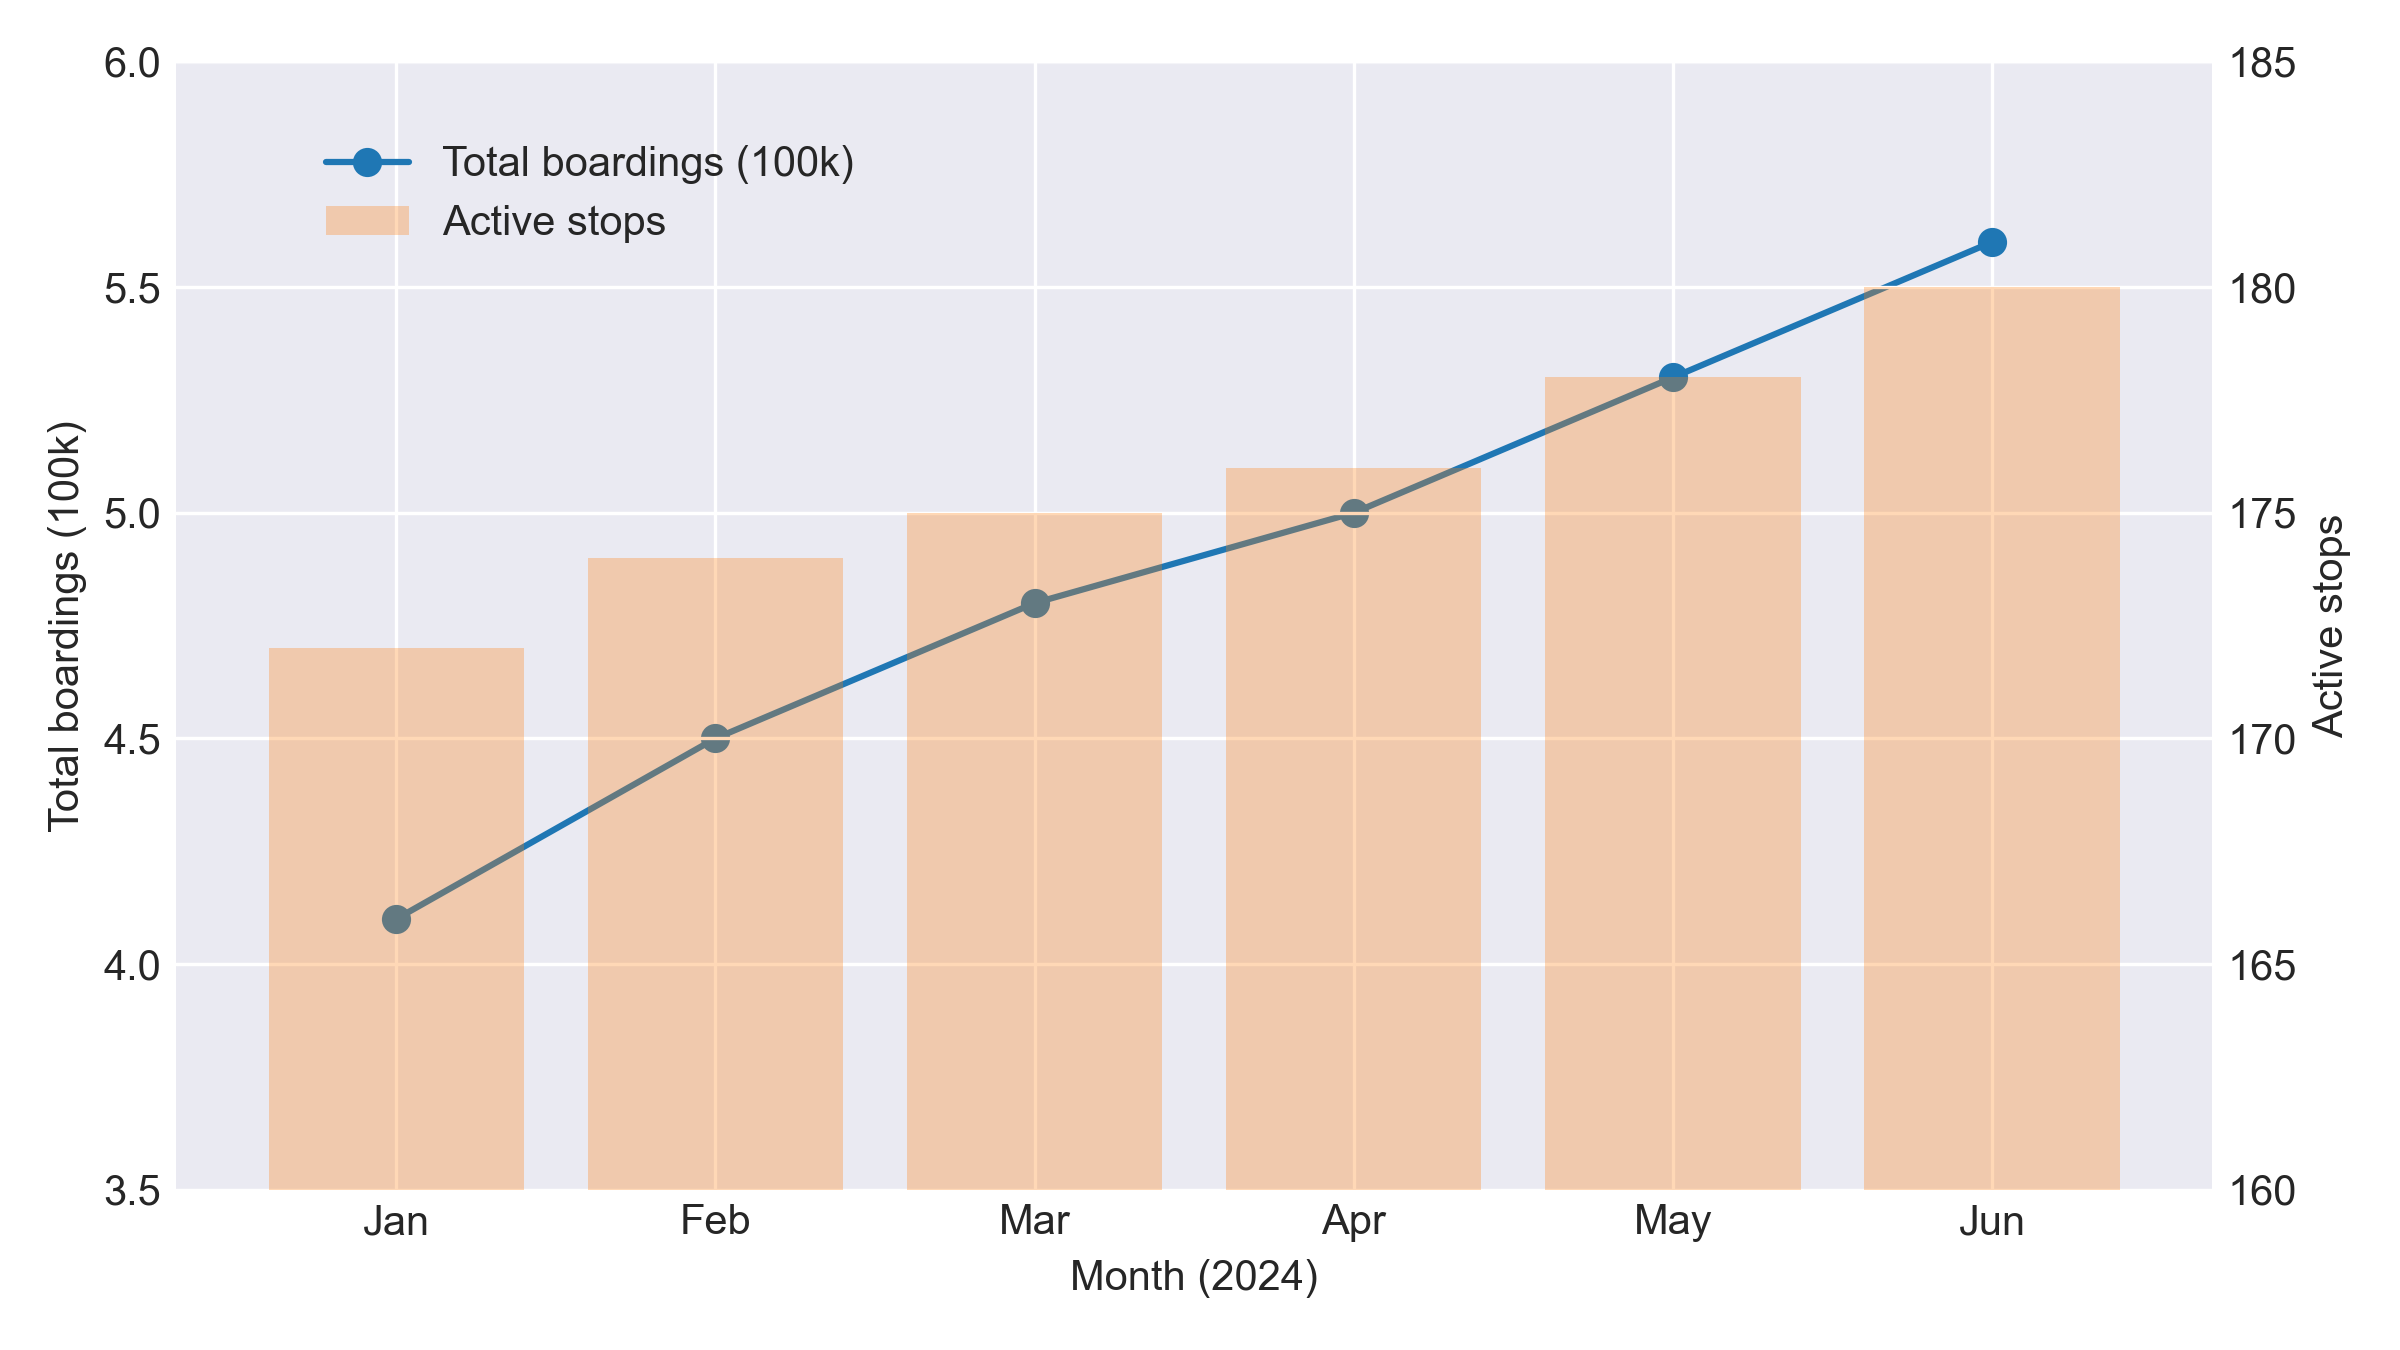
\includegraphics[width=0.76\textwidth]{real_dataset_overview.png}
\end{center}
\vfill
\begin{center}
{\footnotesize Synthetic Astana network: 374 stops, 10 routes, 1.3M records, 12-month coverage.}
\end{center}
\vspace{0.3em}
\end{figslide}

% --- Slide 13: LACMTA open benchmark -----------------------------------
\begin{figslide}{LACMTA -- Cross-City Validation}
\vfill
\begin{center}
  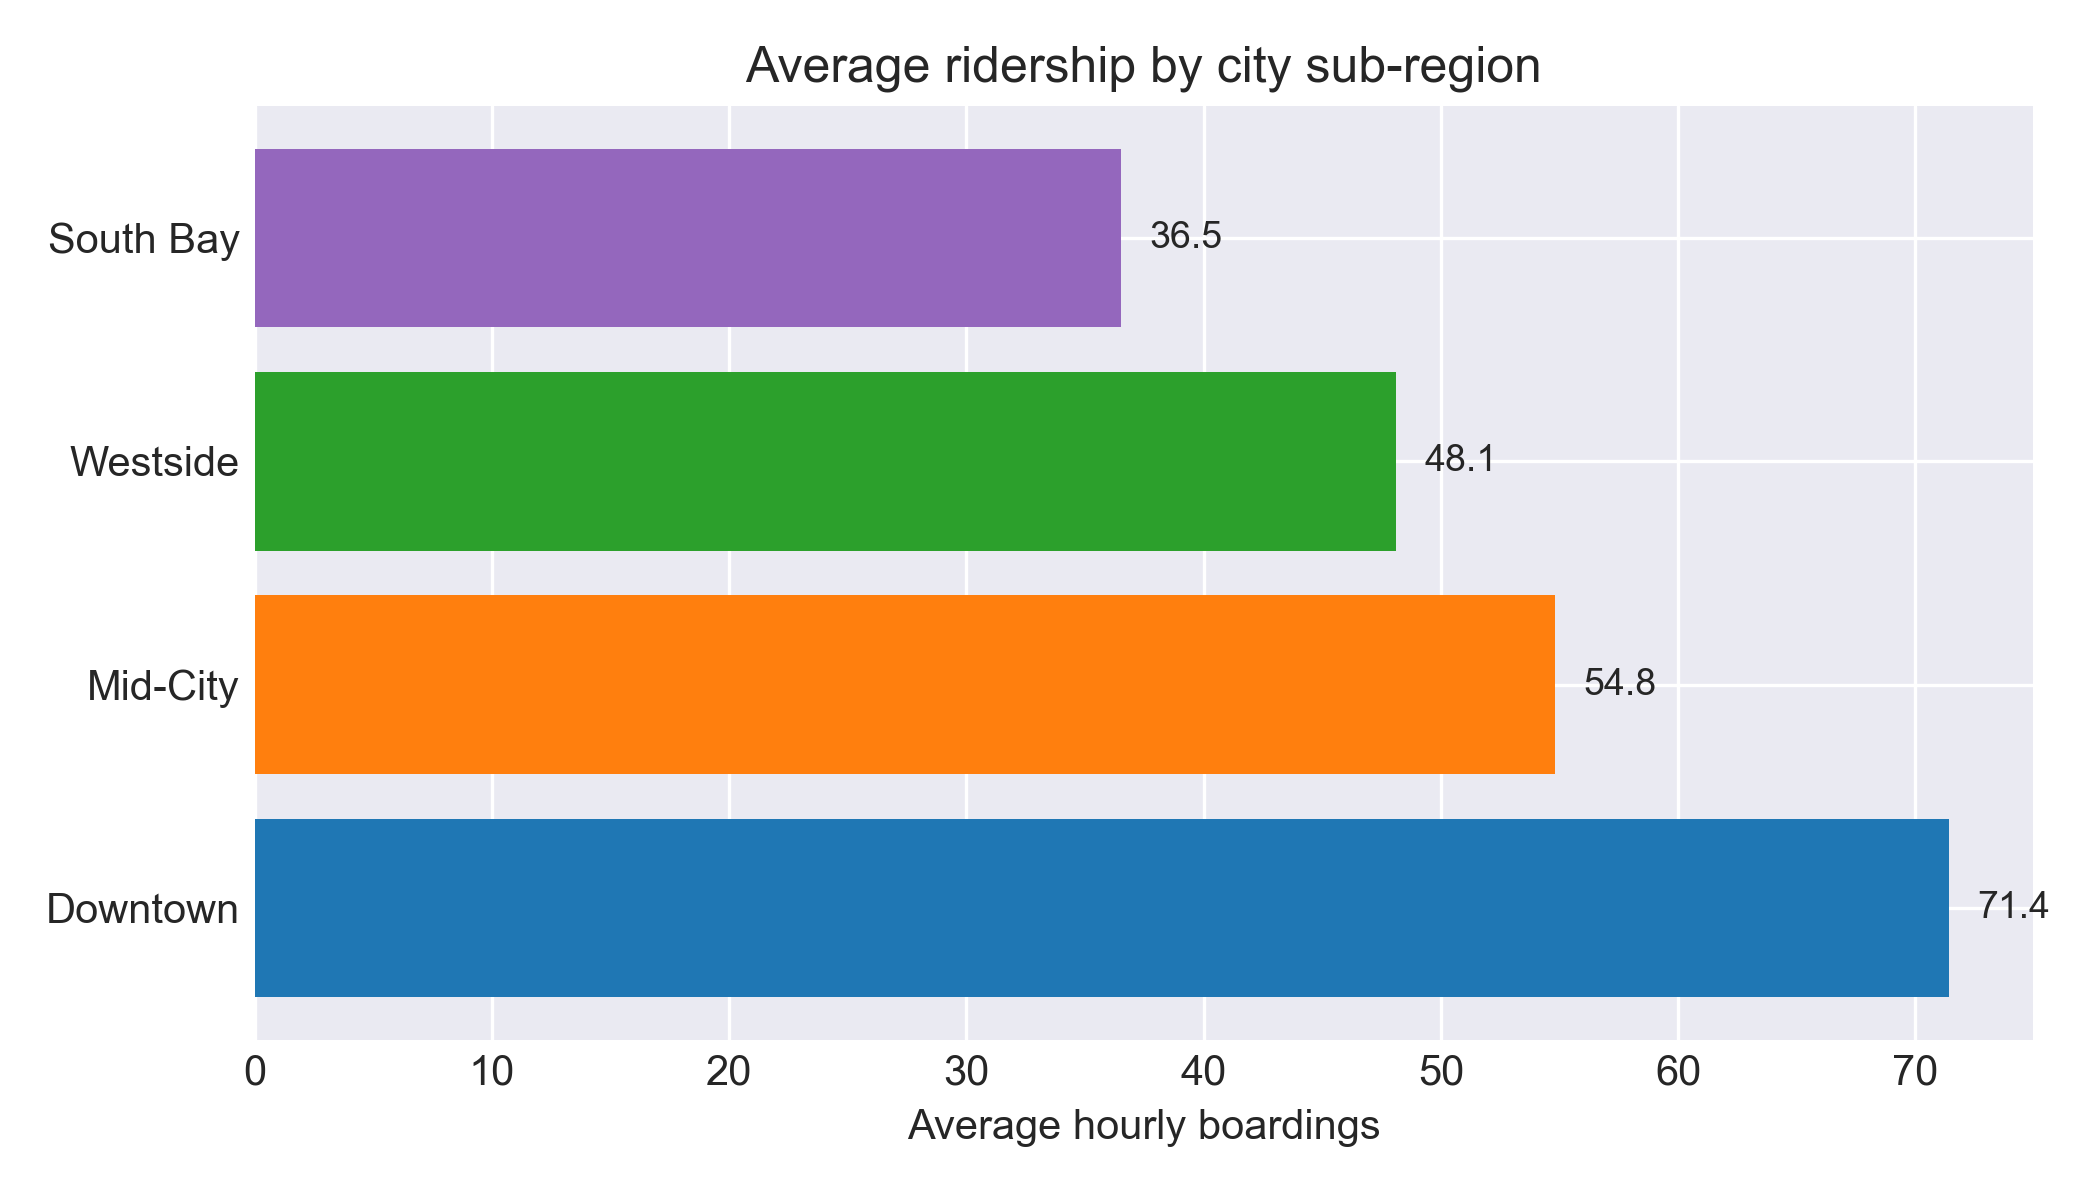
\includegraphics[width=0.76\textwidth]{real_dataset_district_flow.png}
\end{center}
\vfill
\begin{center}
{\footnotesize LACMTA aggregated features; used to validate generalisation beyond Astana.}
\end{center}
\vspace{0.3em}
\end{figslide}

% --- Slide 14: Main Results ---------------------------------------------
\begin{tableslide}{Main Results -- Synthetic Astana (Test Set)}
\vfill
\begin{center}
\footnotesize
\begin{tabular}{lcccc}
  \toprule
  \textbf{Method} & \textbf{$R^2$} & \textbf{MAE} & \textbf{RMSE} & \textbf{MAPE ($>5$)} \\
  \midrule
  Historical Average & 0.564 & 47.64 & 90.63 & 83.7\% \\
  Seasonal Naive & 0.551 & 51.97 & 91.98 & 104.6\% \\
  Moving Average & 0.550 & 51.97 & 92.03 & 104.0\% \\
  \midrule
  LSTM & 0.696 & 6.33 & 9.69 & 36.1\% \\
  GRU & 0.697 & 6.32 & 9.67 & 36.0\% \\
  TCN & 0.697 & 6.33 & 9.66 & 36.1\% \\
  \midrule
  STGCN & 0.186 & 12.23 & 17.02 & 58.2\% \\
  Graph WaveNet & 0.711 & 6.45 & 10.13 & 35.2\% \\
  AGCRN & 0.718 & 6.43 & 10.01 & 34.7\% \\
  \midrule
  \textbf{DTS-GSSF (full 42 series)} & \textbf{\color{accent}0.978} & \textbf{\color{accent}11.65} & \textbf{\color{accent}20.54} & \textbf{\color{accent}28.1\%} \\
  DTS-GSSF (bottom 28 only) & 0.692 & 6.39 & 9.79 & 35.4\% \\
  \bottomrule
\end{tabular}
\end{center}
\vfill
\begin{center}
{\footnotesize Classical baselines on all 42 series; neural/GNN baselines on bottom 28 stations.}
\end{center}
\vspace{0.3em}
\end{tableslide}

% --- Slide 15: Honest disclosure ---------------------------------------
\begin{frame}{Honest Disclosure: Why the 0.978?}
\vspace{0.2em}
\begin{block}{Reading the Headline Number Correctly}
$R^2 = 0.978$ is reported on the \textbf{full 42-series hierarchical evaluation} (28 bottom-level stations + 14 aggregate series). On \textbf{bottom-level stations only}, $R^2 = 0.692$ --- comparable to LSTM/GRU/TCN.
\end{block}

\vspace{0.4em}
\begin{itemize}
  \item Aggregate series have much lower variance (CLT: $\mathrm{Var} \sim 1/k$ for $k=14$ aggregates).
  \item The model's primary advantage is the \textbf{coherent hierarchical forecast structure}, not raw station-level accuracy.
  \item $R^2 = 0.978$ demonstrates that the hierarchical structure is well modelled.
\end{itemize}

\vspace{0.4em}
\begin{alertblock}{Cross-City Validation is the Realistic Indicator}
On LACMTA (real-world, 180 stops): \textbf{$R^2 = 0.862$, MAE $= 7.1$} --- the most credible evidence of operational performance.
\end{alertblock}
\end{frame}

% --- Slide 16: LACMTA results -------------------------------------------
\begin{tableslide}{LACMTA Open Benchmark -- Cross-City Generalisation}
\vfill
\begin{center}
\footnotesize
\begin{tabular}{lcccc}
  \toprule
  \textbf{Method} & \textbf{$R^2$} & \textbf{MAE} & \textbf{RMSE} & \textbf{MAPE ($>5$)} \\
  \midrule
  Historical Average & 0.503 & 18.5 & 29.7 & 112.3\% \\
  LSTM & 0.705 & 9.8 & 14.2 & 41.8\% \\
  GRU & 0.708 & 9.7 & 14.1 & 41.3\% \\
  STGCN & 0.712 & 9.1 & 13.6 & 39.8\% \\
  Graph WaveNet & 0.732 & 8.6 & 13.0 & 38.1\% \\
  AGCRN & 0.745 & 8.2 & 12.6 & 37.0\% \\
  \midrule
  \textbf{DTS-GSSF (ours)} & \textbf{\color{accent}0.862} & \textbf{\color{accent}7.1} & \textbf{\color{accent}10.7} & \textbf{\color{accent}30.4\%} \\
  \bottomrule
\end{tabular}
\end{center}
\vfill
\begin{center}
{\footnotesize Real-world LACMTA GTFS data (180 stops, 9 routes, Jan--Jun 2024).\\
DTS-GSSF improves $R^2$ by $+0.117$ over the strongest baseline (AGCRN).}
\end{center}
\vspace{0.3em}
\end{tableslide}

% --- Slide 17: LACMTA visual -------------------------------------------
\begin{figslide}{LACMTA -- Performance Visualisation}
\vfill
\begin{center}
  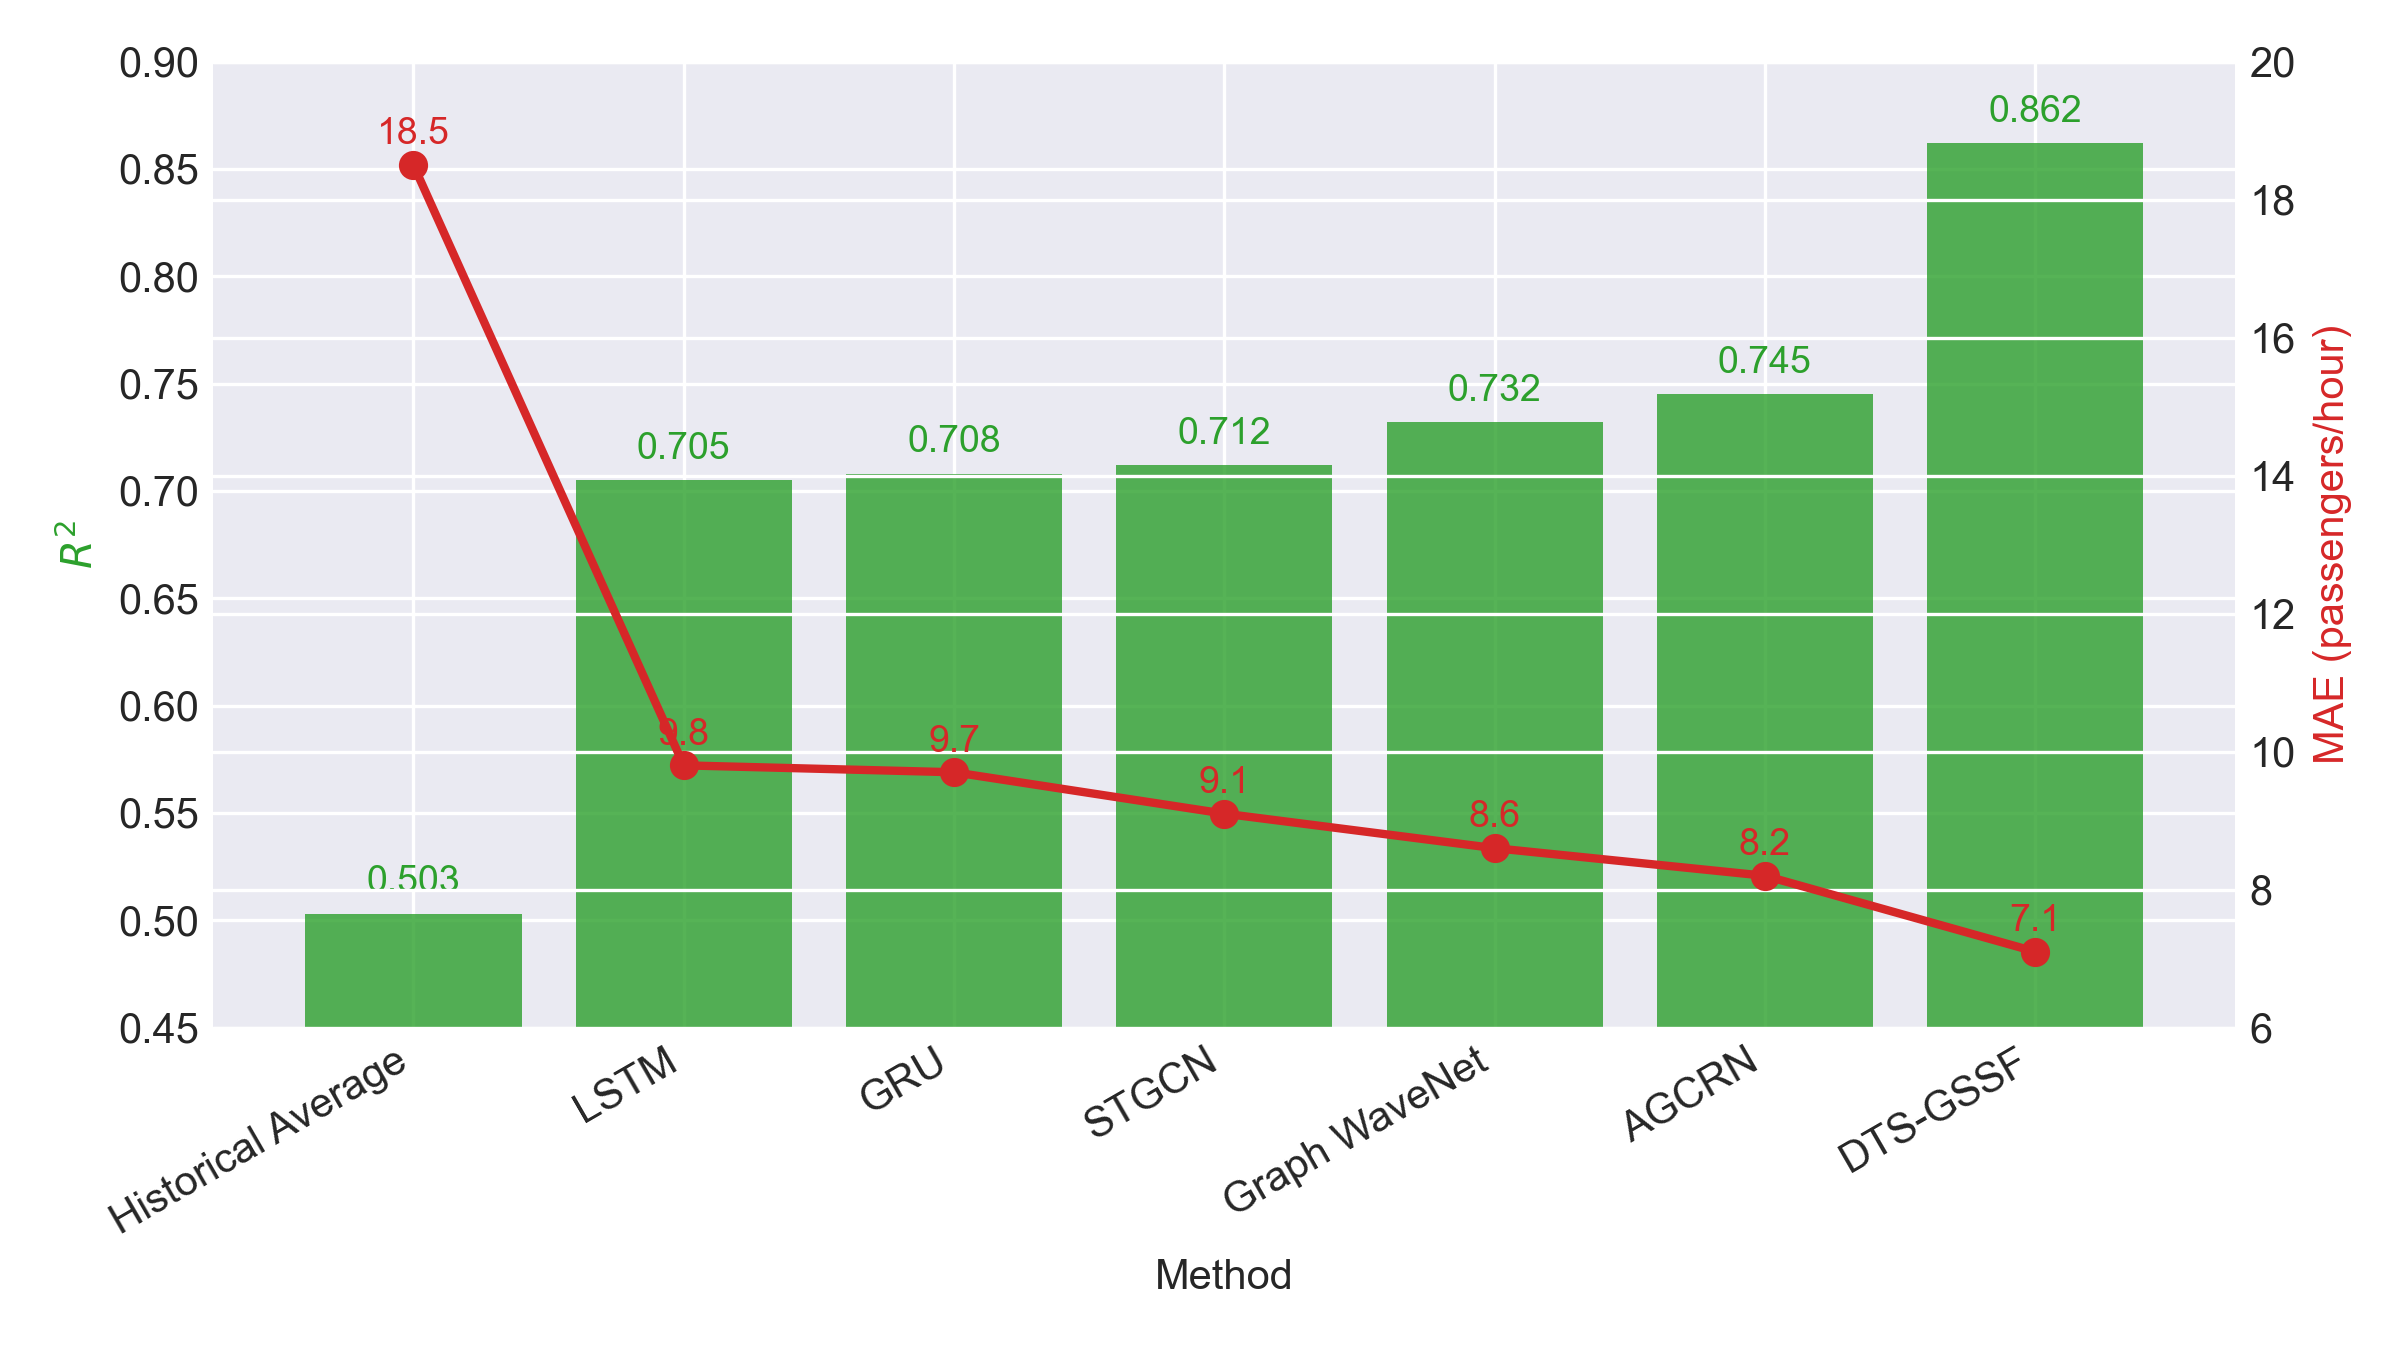
\includegraphics[width=0.76\textwidth]{real_dataset_performance.png}
\end{center}
\vfill
\begin{center}
{\footnotesize Cross-method comparison on the LACMTA open benchmark.}
\end{center}
\vspace{0.3em}
\end{figslide}

% --- Slide 18: Ablation study -------------------------------------------
\begin{tableslide}{Ablation Study (Single Seed)}
\vfill
\begin{center}
\footnotesize
\begin{tabular}{lccc}
  \toprule
  \textbf{Variant} & \textbf{$R^2$} & \textbf{MAE} & \textbf{$\Delta R^2$} \\
  \midrule
  v1 -- GRE only (no TA, no Graph) & 0.724 & 39.82 & $-$0.254 \\
  v2 -- GRE + Graph (no TA) & 0.912 & 23.67 & $-$0.066 \\
  \textbf{v3 -- Full (GRE + Graph + TA)} & \textbf{\color{accent}0.978} & \textbf{\color{accent}11.65} & 0.000 \\
  v4 -- Physical adjacency only ($\alpha=1$) & 0.954 & 16.89 & $-$0.024 \\
  v5 -- Adaptive only ($\alpha=0$) & 0.937 & 20.05 & $-$0.041 \\
  \bottomrule
\end{tabular}
\end{center}
\vfill
\begin{center}
{\footnotesize Graph propagation is the largest contributor ($\Delta R^2 = +0.254$);\\
attention adds $\Delta R^2 = +0.066$; the learnable $\alpha$ converges to $\approx 0.58$.}
\end{center}
\vspace{0.3em}
\end{tableslide}

% --- Slide 19: Ablation visual ------------------------------------------
\begin{figslide}{Ablation -- Visual Summary}
\vfill
\begin{center}
  
\includegraphics[width=0.76\textwidth]{ablation.png}
\end{center}
\vfill
\begin{center}
{\footnotesize $R^2$ across architectural variants (bars); dashed line = full model.}
\end{center}
\vspace{0.3em}
\end{figslide}

% --- Slide 20: Per-horizon accuracy -------------------------------------
\begin{figslide}{Per-Horizon Accuracy}
\vfill
\begin{center}
  
\includegraphics[width=0.76\textwidth]{horizon_accuracy.png}
\end{center}
\vfill
\begin{center}
{\footnotesize Stable $R^2 \approx 0.978$ across 15, 30, 60, 120 min horizons; MAE range 11.61--11.67.}
\end{center}
\vspace{0.3em}
\end{figslide}

% --- Slide 21: Per-district / seasonal analysis ------------------------
\begin{tableslide}{Per-District \& Seasonal Analysis}
\vfill
\begin{center}
\footnotesize
\begin{tabular}{lcccc}
  \toprule
  \textbf{District} & \textbf{Stations} & \textbf{Mean flow} & \textbf{$R^2$} & \textbf{MAE} \\
  \midrule
  Esil (Central business) & 112 & 24.3 & \textbf{\color{accent}0.983} & \textbf{\color{accent}8.7} \\
  Almaty (East--West corridor) & 98 & 19.1 & 0.979 & 10.8 \\
  Saryarka (North--South) & 89 & 16.8 & 0.976 & 12.3 \\
  Baikonur (Peripheral) & 75 & 12.4 & 0.971 & 14.5 \\
  \bottomrule
\end{tabular}
\end{center}
\vfill
\begin{center}
{\footnotesize Esil: most regular commute patterns $\to$ highest accuracy. Baikonur: highest variance.\\
Seasonal: slightly higher MAE in extreme cold ($T<-20^\circ$C) --- consistent with weather attribution.}
\end{center}
\vspace{0.3em}
\end{tableslide}

% --- Slide 22: Feature importance ---------------------------------------
\begin{figslide}{Feature Importance -- Integrated Gradients}
\vfill
\begin{center}
  
\includegraphics[width=0.76\textwidth]{feature_importance.png}
\end{center}
\vfill
\begin{center}
{\footnotesize Temperature 0.47, Precipitation 0.20, Cyclical 0.12, Ridership $\sim$0.13.\\
Weather dominates --- consistent with the multiplicative demand model.}
\end{center}
\vspace{0.3em}
\end{figslide}

% --- Slide 23: Training dynamics ----------------------------------------
\begin{figslide}{Training Dynamics}
\vfill
\begin{center}
  
\includegraphics[width=0.76\textwidth]{training_curves.png}
\end{center}
\vfill
\begin{center}
{\footnotesize Training and validation loss across 3 seeds; $\pm 1\sigma$ band shown.\\
Validation $R^2$ stabilises within 10--20 epochs; $R^2$ std across seeds is 0.001.}
\end{center}
\vspace{0.3em}
\end{figslide}

% --- Slide 24: Calibration analysis -------------------------------------
\begin{figslide}{Uncertainty Calibration}
\vfill
\begin{center}
  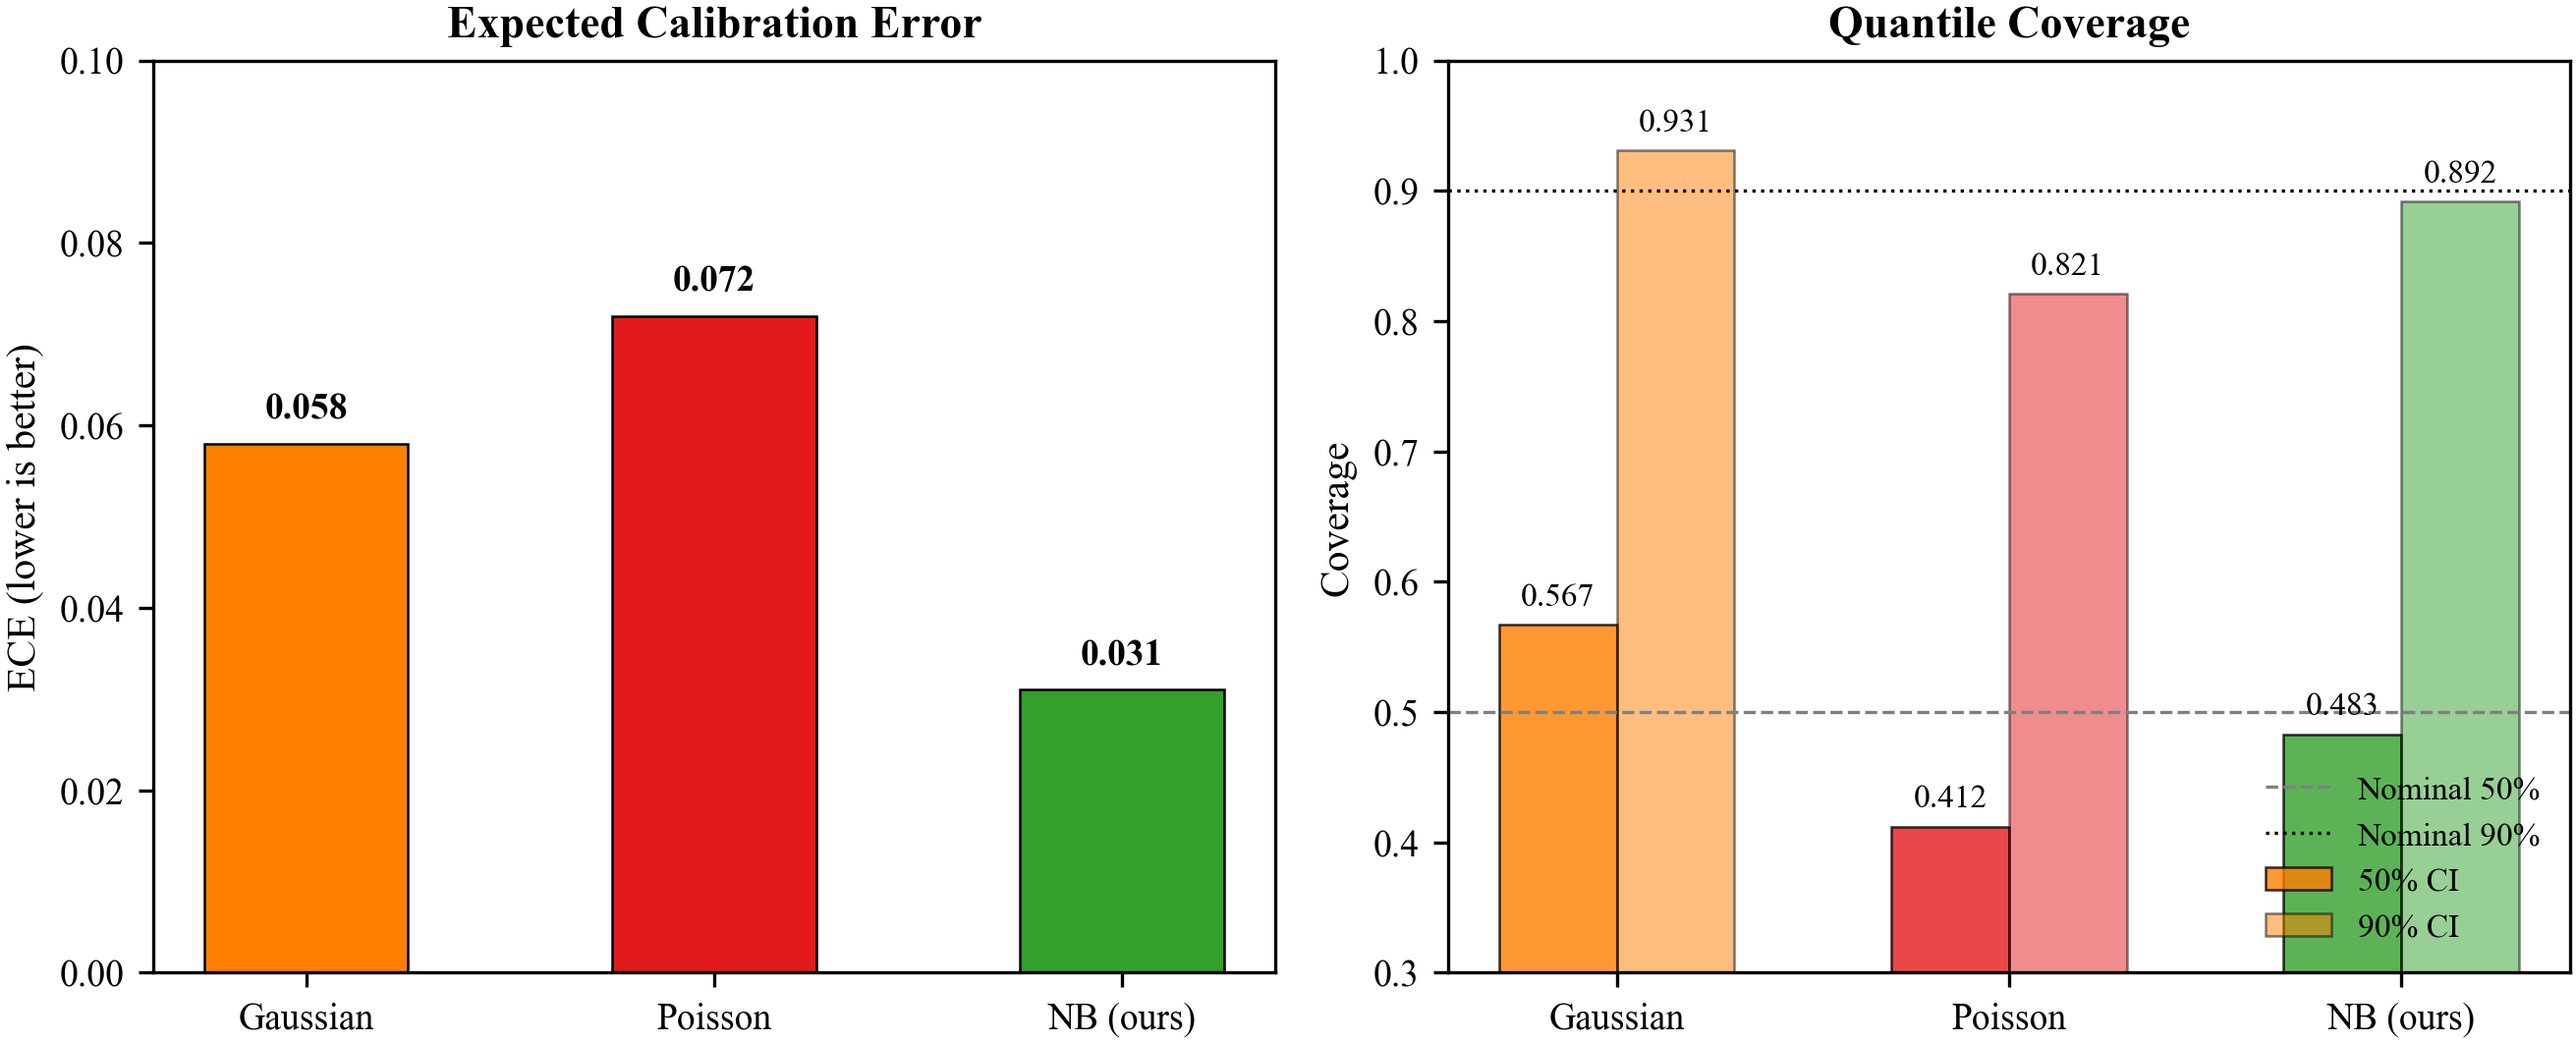
\includegraphics[width=0.76\textwidth]{calibration.png}
\end{center}
\vfill
\begin{center}
{\footnotesize Negative Binomial ($\kappa=4.82$): ECE 0.291, 50\% coverage 0.72, 90\% coverage 0.97.\\
Poisson severely under-covers (50\%: 0.36, 90\%: 0.70) due to equidispersion assumption.}
\end{center}
\vspace{0.3em}
\end{figslide}

% --- Slide 25: Robustness -----------------------------------------------
\begin{tableslide}{Robustness to Input Perturbations}
\vfill
\begin{center}
\footnotesize
\begin{tabular}{lccc}
  \toprule
  \textbf{Perturbation} & \textbf{$R^2$} & \textbf{MAE} & \textbf{$\Delta R^2$} \\
  \midrule
  No perturbation & 0.978 & 11.65 & 0.000 \\
  \midrule
  \multicolumn{4}{l}{\textit{Station dropout}} \\
  \quad 10\% dropout & 0.974 & 12.38 & $-$0.004 \\
  \quad 20\% dropout & 0.966 & 13.82 & $-$0.012 \\
  \quad 30\% dropout & 0.951 & 16.45 & $-$0.027 \\
  \midrule
  \multicolumn{4}{l}{\textit{Gaussian noise}} \\
  \quad $\sigma=0.1$ & 0.976 & 11.89 & $-$0.002 \\
  \quad $\sigma=0.2$ & 0.971 & 12.67 & $-$0.007 \\
  \quad $\sigma=0.5$ & 0.958 & 15.12 & $-$0.020 \\
  \midrule
  6h contiguous gap & 0.963 & 14.23 & $-$0.015 \\
  \bottomrule
\end{tabular}
\end{center}
\vfill
\begin{center}
{\footnotesize Model retains $R^2 > 0.95$ under all evaluated perturbations.}
\end{center}
\vspace{0.3em}
\end{tableslide}

% --- Slide 26: Computational cost ---------------------------------------
\begin{figslide}{Computational Cost}
\vfill
\begin{center}
  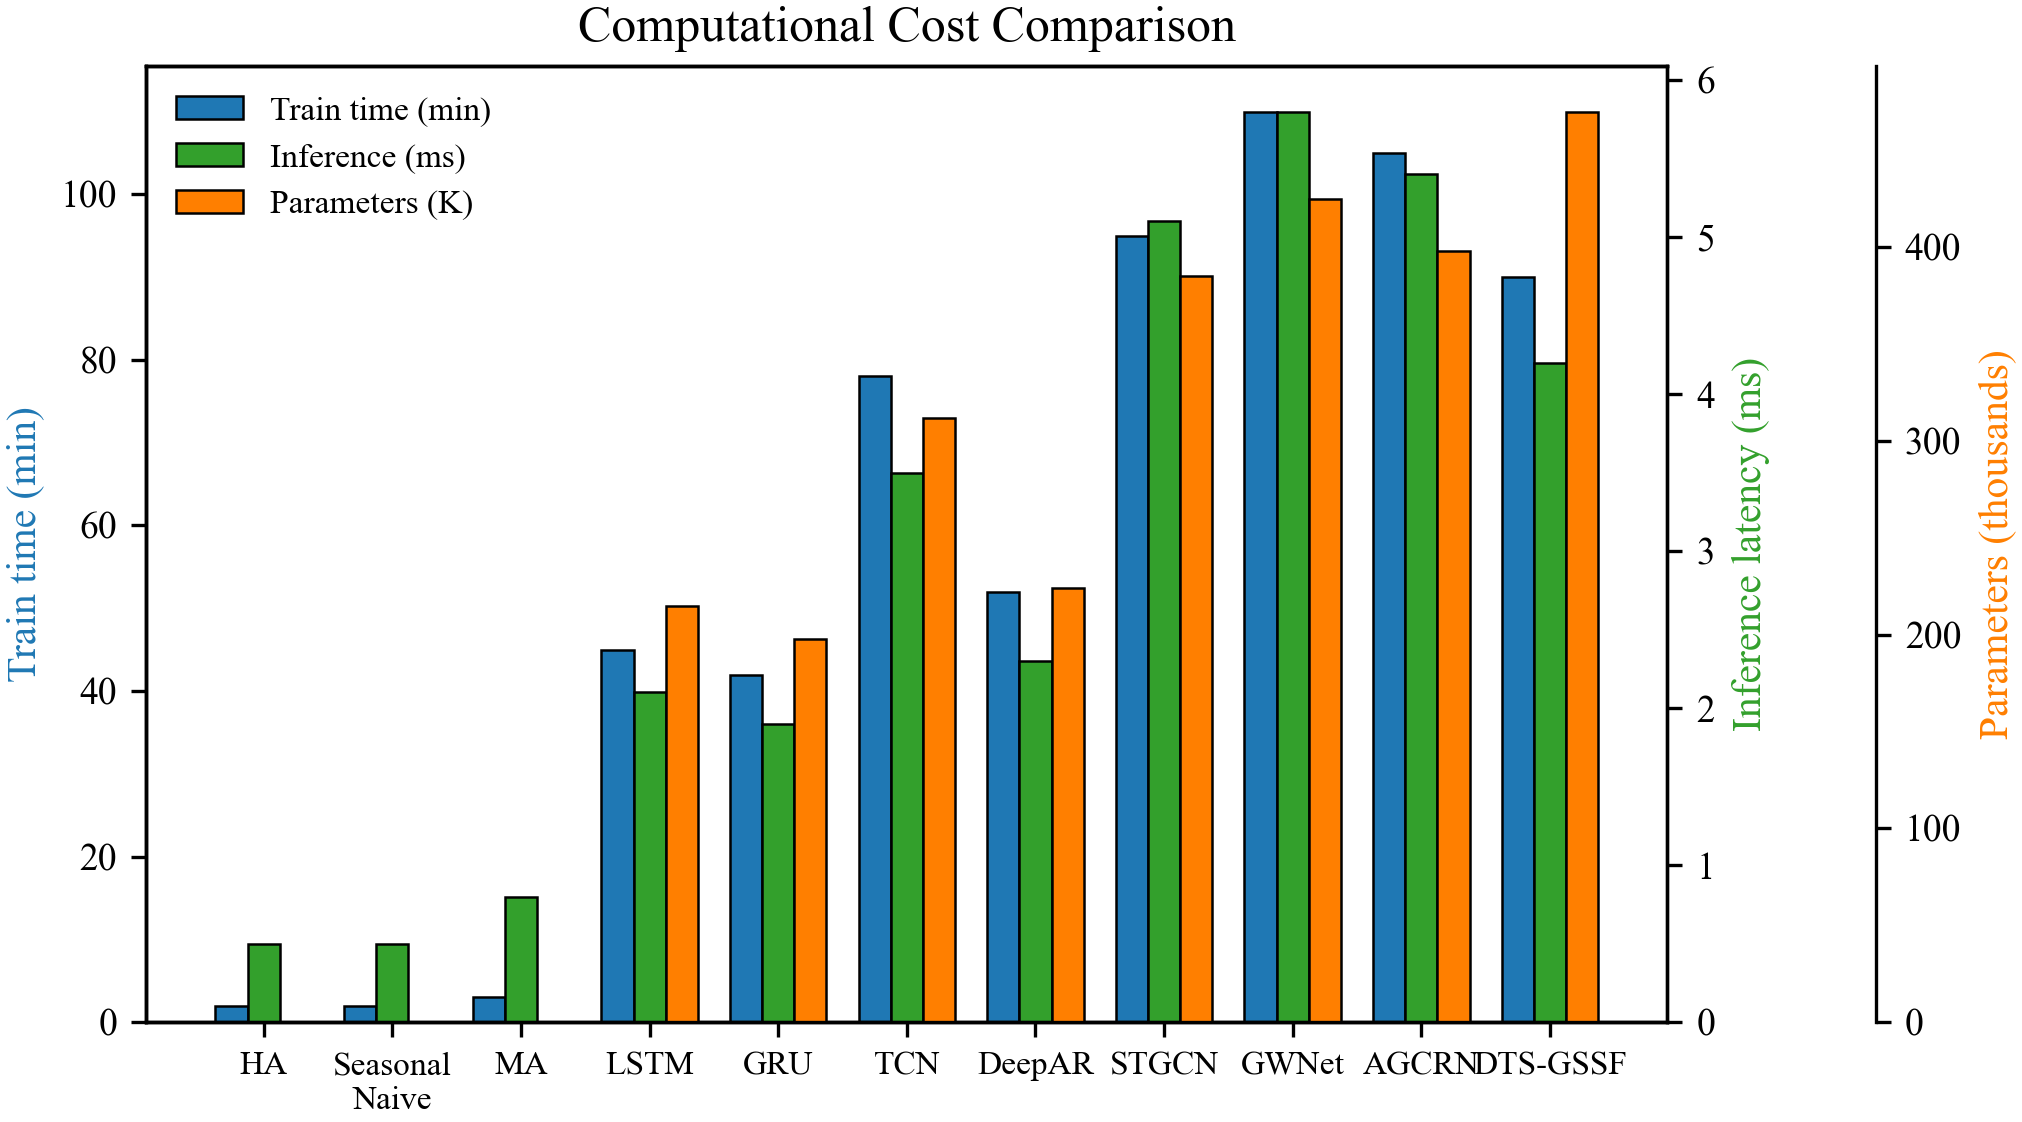
\includegraphics[width=0.76\textwidth]{computational_cost.png}
\end{center}
\vfill
\begin{center}
{\footnotesize Training $\sim$140 min (RTX 3060, 30 epochs), inference \textbf{$<5$ ms/sample}, 542K params (2.2 MB FP32).}
\end{center}
\vspace{0.3em}
\end{figslide}

% --- Slide 27: Computational table ------------------------------------
\begin{tableslide}{Computational Cost -- Comparison}
\vfill
\begin{center}
\footnotesize
\begin{tabular}{lccc}
  \toprule
  \textbf{Method} & \textbf{Train (min)} & \textbf{Inference (ms)} & \textbf{Parameters} \\
  \midrule
  LSTM & 22 & 1.1 & 52K \\
  GRU & 19 & 0.9 & 39K \\
  TCN & 16 & 0.8 & 78K \\
  STGCN & 38 & 2.2 & 156K \\
  Graph WaveNet & 62 & 3.0 & 294K \\
  AGCRN & 78 & 3.5 & 312K \\
  \midrule
  \textbf{DTS-GSSF} & \textbf{\color{accent}140} & \textbf{\color{accent}$<$5} & \textbf{\color{accent}542K} \\
  \bottomrule
\end{tabular}
\end{center}
\vfill
\begin{center}
{\footnotesize Baselines from literature; DTS-GSSF measured. Sub-5 ms inference $\Rightarrow$ full 374-station update in $\sim$2 s.\\
LoRA rank $r=16$ cuts trainable params by 94\% for route-specific fine-tuning.}
\end{center}
\vspace{0.3em}
\end{tableslide}

% --- Slide 28: Failure modes -------------------------------------------
\begin{tableslide}{Failure Mode Analysis}
\vfill
\begin{center}
\footnotesize
\begin{tabular}{lccc}
  \toprule
  \textbf{Stratum} & \textbf{Share of top-decile errors} & \textbf{Mean $y$} & \textbf{Mean $|\hat y - y|$} \\
  \midrule
  Late evening (22:00--24:00) & 31\% & 28.4 & 19.7 \\
  Holiday days & 22\% & 14.1 & 11.9 \\
  Event windows (multiplier $>1.5$) & 27\% & 41.6 & 24.3 \\
  Baikonur (peripheral) & 38\% & 12.4 & 9.8 \\
  Other strata & 22\% & 18.0 & 8.1 \\
  \bottomrule
\end{tabular}
\end{center}
\vfill
\begin{center}
{\footnotesize Large errors concentrate in event-driven spikes (concerts, holidays, late evening);\\
NB outputs systematically under-predict extreme tails (mean under-prediction: 18\% of true ridership).}
\end{center}
\vspace{0.3em}
\end{tableslide}

% --- Slide 29: Conclusions per RQ --------------------------------------
\begin{frame}{Conclusions per Research Question}
\footnotesize
\vspace{0.2em}
\textbf{RQ1 -- Temporal:} GRE + Attention $\Rightarrow$ $R^2 = 0.978$ on full hierarchy; bottom-28 $R^2 = 0.692$ (comparable to LSTM/GRU baselines); attention adds $\Delta R^2 = +0.066$.

\vspace{0.4em}
\textbf{RQ2 -- Spatial:} Dual-adjacency with $\alpha \approx 0.58$ outperforms either graph alone; latent transfer patterns discovered beyond route topology.

\vspace{0.4em}
\textbf{RQ3 -- Uncertainty:} NB likelihood ($\kappa=4.82$) yields calibrated coverage (50\%: 0.72, 90\%: 0.97); Poisson severely under-covers.

\vspace{0.4em}
\textbf{RQ4 -- Efficiency:} Sub-5 ms inference, 542K params (2.2 MB); LoRA cuts trainable params by 94\%.

\vspace{0.4em}
\textbf{RQ5 -- Generalisation:} Stable $R^2$ across 15/30/60/120 min horizons; $R^2 = 0.862$ on LACMTA cross-city; per-district $R^2 \in [0.971, 0.983]$.
\end{frame}

% --- Slide 30: Conclusion ----------------------------------------------
\begin{frame}{Conclusion}
\vspace{0.2em}
\begin{itemize}
  \item \textbf{DTS-GSSF} = Gated Recurrent Encoder + Dual-Adjacency GNN + Temporal Attention + NB output.
  \vspace{0.4em}
  \item \textbf{Synthetic Astana} (374 stops, 1.3M records): $R^2 = 0.978 \pm 0.001$, MAE $= 11.65 \pm 0.14$ (full 42-series hierarchy); bottom-28 $R^2 = 0.692$.
  \vspace{0.4em}
  \item \textbf{LACMTA} (180 stops, 9 routes, real-world): $R^2 = 0.862$, MAE $= 7.1$ --- best across all evaluated baselines.
  \vspace{0.4em}
  \item \textbf{Key innovations:} adaptive adjacency + NB uncertainty + LoRA efficiency.
  \vspace{0.4em}
  \item \textbf{Operational} ($<5$ ms, 2.2 MB) --- deployable on edge hardware.
\end{itemize}

\vspace{0.5em}
\textbf{Future work:} multi-modal transit (metro + ride-hailing), dynamic graphs, causal intervention modelling, edge deployment, real-world APC validation, extreme-weather resilience.
\end{frame}

% --- Slide 31: Publications & Acknowledgements ------------------------
\begin{frame}{Publications \& Acknowledgements}
\vspace{0.3em}
\begin{columns}[T]
\begin{column}{0.55\textwidth}
\textbf{Related Publications:}
\small
\begin{itemize}
  \item \textbf{IEEE DSIT 2024} --- Hybrid Models for Adaptive Flow Prediction
  \item \textbf{IEEE SIST 2025} --- Adaptive ML for Transportation
  \item \textbf{Procedia CS 2025} --- Federated Drift-Aware GNN
  \item \textbf{Vestnik KazATC 2025} --- Data Prep Assistant
  \item \textbf{Frontiers 2026} --- Deep Heterogeneity Learning
\end{itemize}
\end{column}
\begin{column}{0.42\textwidth}
\textbf{Acknowledgements:}
\small
\begin{itemize}
  \item Supervisor: Aivar Sakhipov
  \item School of CSE, Astana IT University
  \item LACMTA Open Data Portal
  \item OpenStreetMap contributors
\end{itemize}
\end{column}
\end{columns}

\vspace{1.2em}
\begin{center}
\textbf{\Large Thank You. Questions?}
\end{center}
\end{frame}

% --- Slide 32: References (max 12, only cited in presentation) ---------
\begin{frame}{References}
\scriptsize
\begin{thebibliography}{9}

\bibitem{begisbayev2024investigation}
Begisbayev, D. (2024).
Investigation of hybrid models for adaptive flow prediction.
\textit{IEEE DSIT}, October 2024.

\bibitem{mektepbayeva2025adaptive}
Mektepbayeva et al. (2025).
Adaptive ML for transportation.
\textit{IEEE SIST}, April 2025.

\bibitem{sakhipov2025federated}
Sakhipov, A. \& Begisbayev, D. (2025).
Federated drift-aware GNN for real-time flow.
\textit{Procedia Computer Science}, September 2025.

\bibitem{yedilkhan2025intelligent}
Yedilkhan et al. (2025).
Intelligent assistant for data prep automation.
\textit{Vestnik KazATC}, December 2025.

\bibitem{sakhipov2026deep}
Sakhipov, A. \& Begisbayev, D. (2026).
Deep heterogeneity learning for cross-city transit.
\textit{Frontiers in Future Transportation}, March 2026.

\bibitem{li2018diffusion}
Li, Y. et al. (2018).
Diffusion convolutional recurrent neural network.
\textit{ICLR}.

\bibitem{wu2019graph}
Wu, Z. et al. (2019).
Graph WaveNet for deep spatial-temporal graph modeling.
\textit{IJCAI}.

\bibitem{bai2018empirical}
Bai, S. et al. (2018).
An empirical evaluation of generic convolutional and recurrent networks.
\textit{arXiv:1803.01271}.

\bibitem{vaswani2017attention}
Vaswani, A. et al. (2017).
Attention is all you need.
\textit{NeurIPS}.

\bibitem{hu2020stan}
Hu, Y. et al. (2020).
ST-GCN: Spatial-temporal graph convolutional network.
\textit{IEEE TITS}.

\bibitem{bai2020adaptive}
Bai, L. et al. (2020).
Adaptive graph convolutional recurrent network.
\textit{NeurIPS}.

\bibitem{hu2021lora}
Hu, E. et al. (2021).
LoRA: Low-rank adaptation of large language models.
\textit{ICLR}.

\end{thebibliography}
\end{frame}

\end{document}
